\documentclass{article}
\usepackage[utf8]{inputenc}
\usepackage{graphicx}
\graphicspath{ {./images/} }
\usepackage{amsmath}
\usepackage{hyperref}
%\usepackage[english]{babel}
\usepackage{pdfpages}

\usepackage{chemfig}

\usepackage[left=2cm,right=1cm, top=2cm,bottom=2cm,bindingoffset=0cm]{geometry}
\renewcommand{\normalsize}{\fontsize{14}{18pt}\selectfont}
\newcommand{\specialcell}[2][c]{%
	\begin{tabular}[#1]{@{}c@{}}#2\end{tabular}}
\renewcommand{\normalsize}{\fontsize{14}{18pt}\selectfont}

\title{Studying  fermentation via RNA-seq  }
\author{ Ignat Sonets, Kamilla Faizullina}
\date{\empty}

\begin{document}
	
		\catcode`\_=\active
	\catcode`\^=\active
	
\maketitle
 We analyze RNA-seq data from yeast  to study gene expression   during fermentation. We make alignment and analyze expressions level using utilities. Using The Saccharomyces Genome Database, we propose the gene which could be important for fermentation process. 
 
\section{Introduction}
 
 Hello! Today we perform differential expression analysis for RNA-seq data of S.cerevisiae to estimate changes in gene expression levels while baking the bread. But before we start, I want to briefly introduce some data about yeasts and fermentation process.
 As we all  know, for making bread we use yeasts. Yeasts eat sugars and put dough to rise. But what processes occur? First, it is an anaerobic process. You might be surprised, but yeasts undergo ethanol fermentation during dough rising (and if you make your dough with more water and leave your mixture near a heat source for about 2-3 days, you will recreate the ancient beer recipe, as it was done by ancient Egyptians.). Fermentation of sugars in flour is the core of bread making. How fermentation works? Ethanol fermentation transforms one mole of glucose into two moles of ethanol and two moles of carbon dioxide (which is the most important component for bread making), producing two moles of ATP (unfortunately, it won't make bread a Red Bull) in the process. 
 Details about given process are taken from \cite{1}.
 The overall chemical formula for alcoholic fermentation is:
 
 \chemfig{C6H12O6  $\rightarrow$ 2 C2H5OH + 2 CO2}
 
 Sucrose is a sugar composed of a glucose linked to a fructose. In the first step of alcoholic fermentation, the enzyme invertase cleaves the glycosidic linkage between the glucose and fructose molecules.(NB: almost the same process can be made with saccharose, which is also dimer consist of glucose and fructose, but with different glycoside bond).
 
 \ce{C12H22O11 + H2O + invertase → 2 C6H12O6}
 
 Next, each glucose molecule is broken down into two pyruvate molecules in a process known as glycolysis \cite{2}. Glycolysis is summarized by the equation:
 
 C6H12O6 + 2 ADP + 2 Pi + 2 NAD+ → 2 CH3COCOO− + 2 ATP + 2 NADH \\
 + 2 H2O + 2 H+
 
 CH3COCOO− is pyruvate, and Pi is inorganic phosphate. Finally, pyruvate is converted to ethanol and CO2 in two steps, regenerating oxidized NAD+ needed for glycolysis:
 
 1. CH3COCOO− + H+ → CH3CHO + CO2
 
 catalyzed by pyruvate decarboxylase
 
 2. CH3CHO + NADH + H+ → C2H5OH + NAD+
 
 This reaction is catalyzed by alcohol dehydrogenase.
 So, we think, that yeasts would behave differently between 2 states: before the start of the fermentation and during the fermentation, because cells will(and should) respond to its changing environment. To provide necessary enzymes for fermentation, the yeast cell should start their synthesis (i.e. translation). To start their synthesis, transcription (DNA to RNA information transfer) should begin. So your gene expression(i.e. the process by which information from a gene is used in the synthesis of a functional gene product that enables it to produce protein as the end product\cite{3}) changes. But how to e s t i m a t e this? Differential expression analysis at your service. To do this, we need RNA-seq data, reference genome of S.cerevisiae, annotation file (to find which gene changed its expression levels) and skills. By measuring differences in gene expression we can not only confirm our suggestions, but also discover new data that could potentially be useful in biotechnology(i.e. modifying enzymes, maybe adding new enzymes or even massive genomic rearrangements) and even on your kitchen by, for example, tweaking flour/water proportions, changing flour type, adding more sugar etc. This could be done with tries and errors and many repeats, but if we can obtain some evidence-based discoveries, why not?
 Let's get started.
 
 
 \section{Data}
We analyze transcriptome data of Saccharomyces cerevisiae
obtained using IconIllumina HiSeq 2000.   In order to study RNA expression levels, we use RNA-seq data from yeast obtained before and during fermentation \cite{data}. 

We also use Saccharomyces cerevisiae assembly R64  strain S288C from NCBI \cite{ncb} as a reference genome data. The data were obtained via  	Illumina HiSeq 2000.  %This is a species of yeast. 


\section{Methods}
 RNA-seq differential gene expression analysis allows to measure  quantitative changes in the expression levels between the experiments.  We analyze yeast data before and during fermentation as we would like to compare expression of  different genes between  fermentation process and normal growth. 
 
 First, we should make alignment. We use HISAT2 which allows us make  alignment  for RNA sequencing reads \cite{hisat}. HISAT2 alignment is based on extended the Burrows-Wheeler transform  with indexing sequences. 
 
 The utility DESeq2 is used to perform differential gene expression analysis \cite{deseq}. This method is based on the assumption  negative binomial distribution in the model. We use command $\textrm{featureCounts}$ from the Subread package \cite{featurecounts} for counting reads and command $\textrm{gffread}$ \cite{gff} to prepare results for DESeq2. 
 
 After using DESeq2, we have output results. To visualize RNA-Seq results, we can use heatmap plots and volcano plots \cite{volcano}.   
 
   To make interpretation of results, we use Saccharomyces Genome Database  by Stanford \cite{ontology}. The Saccharomyces Genome Database provides information about genes functions  from the yeast genome. 
 
 
 \section{Results}
 
 	We successfully aligned  our data to S288C reference genome using HISAT. Results are in Table 1.
 
 
 	\begin{table}[h!]
 	\centering
 	\begin{tabular}{|c|c|c|c|c|}
 		\hline
 		Reads & SRR941816& SRR941817 & SRR941818 & SRR941819  \\
 		\hline
 	 Assigned	& 7291723&	7987001	&1402166	& 4975466 \\
 		\hline
 		 Unassigned-Unmapped &	520138 & 	511726&	66371	& 234531\\
 		\hline
  
 	\end{tabular}
 	\caption{  HISAT alignment results short summary }
 	\label{tab:2}
 \end{table}
 
 Later we filtered and sorted our results using SAMtools. After coverting GFF annotation file to GTF, we used FeatureCounts to count reads for various genes and features. DESEQ2 package outputs gave us normalized counts for each feature, and heatmap(Fig. 1) shows us 1)clustering of two states (0 min/30 min) and 2)difference of gene expression between 2 states (the more red point is, the bigger the value and so the bigger is expression).To put in simplified way, when observing the heatmap we can see that across all genes, proprotion of expressed genes of 0 min/30 min are approx. 50/50, and genes which are expressed in 0 min state are not expressed in 30 min state. 
 
 
  \begin{figure}[h]
 	\centering
 	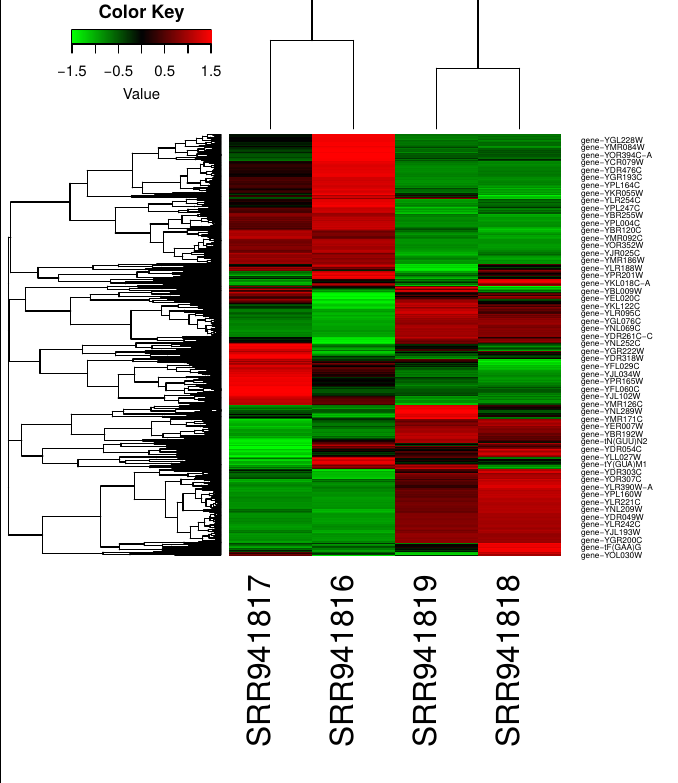
\includegraphics[scale=1.77]{heatmap}  
 	\caption{ Heatmap of differentially expressed genes made with DESEQ2 results.}
 	\label{heatmap}
 \end{figure}
 
 
 Finally, GO Slim mapper was used to "attach" top 50 genes with lowest adjusted p-value(so the most important observations were selected) for corresponding metabolics pathway(See Suppl.Table 1 for more info)
 To visulaize up/downregulation of the genes according to organism state(before/strat fermentaion), we made a volcano plot showing all of 50 genes.
 
 \begin{figure}[h]
	\centering
	\includegraphics[scale=0.47]{tree}  
	\caption{ Volcano plot showing top-50 up/downregulated genes.}
	\label{tree}
\end{figure}
 
 In total(according p-adj. value) 3450 gene changed its expression before starting the fermentation and after 30 min of fermentation. But describing each of the changes would take an eternity, so we narrowed down the focus to top 50 genes. We found 39 GO terms describing these pathways (see Suppl.Table 1 for more details.), and all of them are upregulated. According to the volcano plot, 48 out of 50 genes are upregulated (see Fig.\ref{tree}), except for 2 genes.
  
 The main reason for such a result is a need for fast adaptation for new conditions, main limitaion of them(these new conditions) is lack of O2, and to survive, yeast cell should assemble ribosomes, create a lot of new RNAs of all types, assemble new enzymes, transport new sugars and start converting them to ATP as fast as possible. And we can clearly see, that is happening exactly as we predicted. Let's investigate GO terms and genes more thoroughly.
 
 We start with downregulrated genes, because there are only 2 of them. First, YKR097W (PCK1)\cite{11} . This gene belongs to carbohydrate metabolic process term ( GO:0005975 ). This gene encodes phosphoenolpyruvate carboxykinase; it is the key enzyme in gluconeogenesis, catalyzes early reaction in carbohydrate biosynthesis, located in the cytosol. By switching metabolism to sugars degradation in lack of O2, gluconoegenesis is not needed, so no surprise it is downregulated. One can assume that gene is essential for gluconeogenesis which is crucial when growing on sugars-free media, but flour is rich for carbohydrates, so no senese in this gene and its product during bread making. 
 
 
 The second gene--YLR327C(TMA10)\cite{21}  -- is not allocated for any of GO terms. It encodes protein of unknown function that associates with ribosomes; it is known that protein abundance increases in response to DNA replication stress. Here things got more speculative. At first glance, ribosomes number should rise (as bread:) ), and so this protein should also produce more active, but we don't see this. So I can't give the exact answer that could reveal role of this protein. The only thing I can assume that this protein forms dimeric complexes with ATP-synthase (Dienhart M, et al. (2002)\cite{31} ). As we all know, fermentation is much less energy-efficient than aerobic metabolism,so cell doesn't nedd so much ATP-synthases units,and numbers of TMA10 and TMA10 RNA decreases.
 
 Other genes are upregulating, and because we can't discuss all of 48 genes and their roles in pathways, we will choose only 1 gene and try to hypothesize how it might be a part of actual changes in yeast metabolism. For example, SYO1 / YDL063C \cite{41}, part of the ribosomal large subunit biogenesis (GO:0042273). It is SYnchronized impOrt or SYmpOrtin ; it is assembly chaperone that co-translationally associates with nascent Rpl5p, preventing aggregation; facilitates synchronized nuclear coimport of two 5S-rRNA binding proteins, Rpl5p and Rpl11p, mediated by import receptor Kap104p; required for biogenesis of the large ribosomal subunit. By helping with an assembly of LSU (5S rRNA is a structural component of LSU), thus accelerating ribosome assembly as a functional complex, it provides the synthesis of necessary enzymes and maintaining fermentation speed and keeping the cell alive.
 Thank you for your attention!
 
 
%\newpage 
%\newpage 
\begin{thebibliography}{9}
	\bibitem{1} https://en.wikipedia.org/wiki/Ethanol_fermentation#Biochemical_process_of_fermentation_of_sucrose



	\bibitem{2}	
	Stryer, Lubert (1975). Biochemistry. W. H. Freeman and Company. ISBN 978-0-7167-0174-3.
	
		\bibitem{3}
		https://en.wikipedia.org/wiki/Gene_expression
	
	
 \bibitem{data}

ftp.sra.ebi.ac.uk/vol1/fastq/SRR941/SRR941816/SRR941816.fastq.gz 

ftp.sra.ebi.ac.uk/vol1/fastq/SRR941/SRR941817/SRR941817.fastq.gz 

 ftp.sra.ebi.ac.uk/vol1/fastq/SRR941/SRR941818/SRR941818.fastq.gz 
 
 ftp.sra.ebi.ac.uk/vol1/fastq/SRR941/SRR941819/SRR941819.fastq.gz (282 Mb)

 \bibitem{ncb}
 Sayers EW, Agarwala R, Bolton EE, Brister JR, Canese K, Clark K, Connor R, Fiorini N, Funk K, Hefferon T, Holmes JB, Kim S, Kimchi A, Kitts PA, Lathrop S, Lu Z, Madden TL, Marchler-Bauer A, Phan L, Schneider VA, Schoch CL, Pruitt KD, Ostell J. Database resources of the National Center for Biotechnology Information. Nucleic Acids Res. 2019 Jan 8;47(D1):D23-D28. doi: 10.1093/nar/gky1069. PubMed PMID: 30395293; PubMed Central PMCID: PMC6323993. 2: Sayers EW, Cavanaugh M, Clark K, Ostell J, Pruitt KD, Karsch-Mizrachi I. GenBank. Nucleic Acids Res. 2019 Jan 8;47(D1):D94-D99. doi: 10.1093/nar/gky989. PubMed PMID: 30365038; PubMed Central PMCID: PMC6323954.
 
 
 
\bibitem{hisat}
Kim D, Langmead B and Salzberg SL. HISAT: a fast spliced aligner with low memory requirements. Nature Methods 2015

\bibitem{deseq}
Love MI, Huber W, Anders S (2014). “Moderated estimation of fold change and dispersion for RNA-seq data with DESeq2.” Genome Biology, 15, 550. doi: 10.1186/s13059-014-0550-8. 


\bibitem{featurecounts}
Liao Y, Smyth GK and Shi W (2014).  featureCounts:  an efficient general pur-pose program for assigning sequence reads to genomic features.Bioinformatics,30(7):923-30.http://www.ncbi.nlm.nih.gov/pubmed/24227677

\bibitem{gff}
How to cite this article
Pertea G and Pertea M. GFF Utilities: GffRead and GffCompare [version 1; peer review: 3 approved]. F1000Research 2020, 9:304 (https://doi.org/10.12688/f1000research.23297.1) 

\bibitem{volcano}
Maria Doyle, 2021 Visualization of RNA-Seq results with Volcano Plot (Galaxy Training Materials). /training-material/topics/transcriptomics/tutorials/rna-seq-viz-with-volcanoplot/tutorial.html Online; accessed Fri Apr 02 2021

\bibitem{ontology}
Cherry JM, Hong EL, Amundsen C, Balakrishnan R, Binkley G, Chan ET, Christie KR, Costanzo MC, Dwight SS, Engel SR, Fisk DG, Hirschman JE, Hitz BC, Karra K, Krieger CJ, Miyasato SR, Nash RS, Park J, Skrzypek MS, Simison M, Weng S, Wong ED (2012) Saccharomyces Genome Database: the genomics resource of budding yeast. Nucleic Acids Res. Jan;40(Database issue):D700-5. [PMID: 22110037]

 
 \bibitem{11}
 https://www.yeastgenome.org/locus/YKR097W
 
\bibitem{21}
https://www.yeastgenome.org/locus/S000004319

\bibitem{31}
 Dienhart M, et al. (2002) Formation of the yeast F1F0-ATP synthase dimeric complex does not require the ATPase inhibitor protein, Inh1. J Biol Chem 277(42):39289-95

\bibitem{41} 
https://www.yeastgenome.org/locus/YDL063C

\end{thebibliography}

  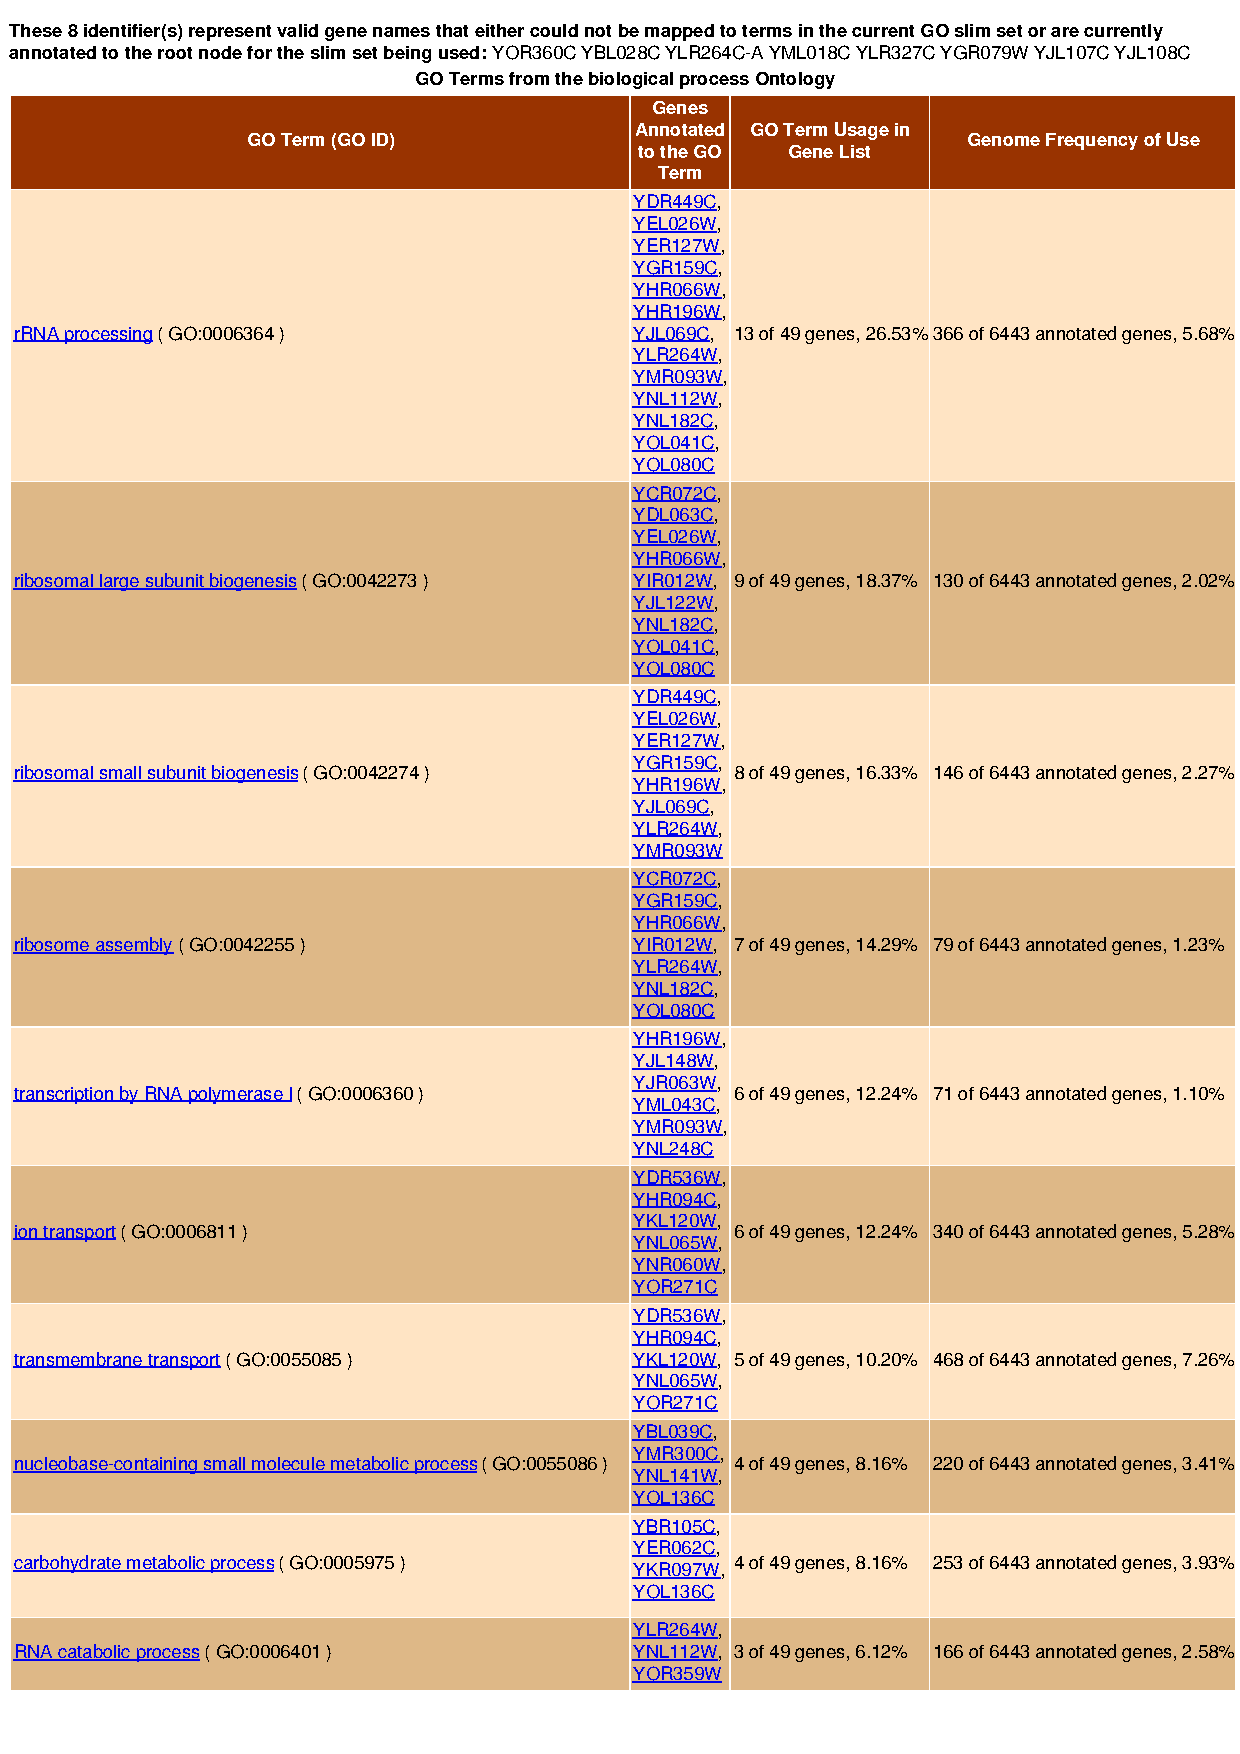
\includepdf[pages=-]{genes.pdf}


\end{document}
